\documentclass{standalone}
\usepackage{tikz}
\usetikzlibrary{shapes, arrows, positioning}
\begin{document}
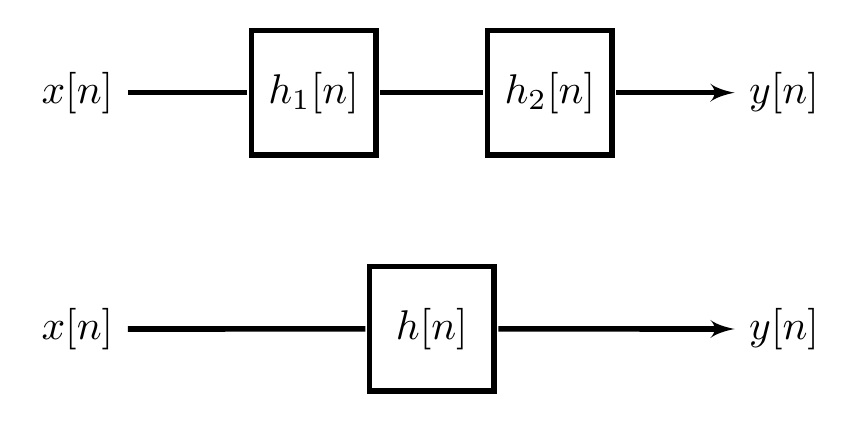
\begin{tikzpicture}[auto,>=latex', transform shape, scale=1.5]

\tikzstyle{block} = [draw, shape=rectangle, minimum height=3em, minimum width=3em, node distance=2cm, line width=2pt]

%Creating Blocks and Connection Nodes
\node at (0,0) (in1) {$x[n]$};
\node [block, right of=in1] (h1) {$h_1[n]$};
\node [block, right of=h1] (h2) {$h_2[n]$};
\node [right = of h2] (out1) {$y[n]$};
\path (h1) -- coordinate (mid) (h2);
\node [block, below of = mid] (h) {$h[n]$};
\node at (in1 |- h) (in2) {$x[n]$};
\node at (out1 |- h) (out2) {$y[n]$};

%Conecting Blocks
\draw[->, line width=2pt] (in1) -- (h1) -- (h2) -- (out1);
\draw[->, line width=2pt] (in2) -- (h) -- (out2);
\end{tikzpicture}
\end{document}
